
\documentclass[11pt]{article}
\usepackage[paper=letterpaper, margin=.5in]{geometry}
\pdfpagewidth 8.5in
\pdfpageheight 11in
\setlength\parindent{0in}

%%% Packages
% First four - AMS (american mathematical society). General math goodness. I use the align* enviorment in particular
% multirow, multicol allow for certain kinds of tables
% enumerate lets you determine the style of the counter for the enumerate enviorment
% graphicx lets you include pictures
% listings lets you stick in blocks of code
% placeins defines "\FloatBarrier", which stops tables from moving around
\usepackage{amsmath, amscd, amssymb, amsthm, multirow, multicol, enumerate, graphicx, listings, placeins} 
\newcommand{\Z}{\mathbb{Z}}
\newcommand{\R}{\mathbb{R}}
\newcommand{\Q}{\mathbb{Q}}
\newcommand{\C}{\mathbb{C}}
\newcommand{\N}{\mathbb{N}}
\newcommand{\V}{\mathbb{V}}
\newcommand{\U}{\mathcal{U}}
\newcommand{\del}{\partial}
\newcommand{\real}{\textrm{Re }}
\newcommand{\imag}{\textrm{Im }}
\newcommand{\pd}[2]{\frac{\partial #1}{\partial #2}}
\newcommand{\deriv}[2]{\frac{d #1}{d #2}}
\newcommand{\sumk}{\sum_{k=1}^\infty}
\newcommand{\sumj}{\sum_{j=1}^\infty}
\newcommand{\sumn}{\sum_{n=0}^\infty}
\newcommand{\summ}[2]{\sum_{k=#1}^{#2}}
\newcommand{\sig}[1]{\sum_{#1 =1}^\infty}
\newcommand{\un}[1]{\bigcup_{#1 =1}^\infty}
\newcommand{\inter}[1]{\bigcap_{#1 =1}^\infty}
\newcommand{\ip}[2]{\langle #1, #2 \rangle}
\newcommand{\ipxu}{\langle x,u_j \rangle}
\newcommand{\uj}{\{u_j\}_{j=1}^\infty}
\newcommand{\B}{\mathcal{B}}

\newcommand{\E}{\mathrm{E}}
\newcommand{\var}{\mathrm{Var}}
\newcommand{\cov}{\mathrm{Cov}}
\newcommand{\ST}{mbox{ s.t. }}

\newcommand{\Example}{\noindent {\bf Example. \quad} }
\newcommand{\Proof}{\noindent {\bf Proof: \quad} }
\newcommand{\Remark}{\noindent {\bf Remark. \quad} }
\newcommand{\Remarks}{\noindent {\bf Remarks. \quad} }
\newcommand{\Case}{\noindent {\underline{Case} \quad} }

\newcommand{\st}{ \; \big | \:}

\newcommand{\deuc}{d_{\mathrm euc}}
\newcommand{\dtaxi}{d_{\mathrm taxi}}
\newcommand{\ddisc}{d_{\mathrm disc}}
\newtheorem{theorem}{Theorem}[section]
\newtheorem{lemma}[theorem]{Lemma}
\newtheorem{proposition}[theorem]{Proposition}
\newtheorem{corollary}[theorem]{Corollary}
\theoremstyle{definition}
\newtheorem{definition}[theorem]{Definition}
\newtheorem{example}[theorem]{Example}

\begin{document}
%%%%%%%%%%%%%%%%%%%%%%%%%%%%%%%%%%%%%%%%%%%%%%%%%%%%%%%%%%%%%%%%%%%%%%%%%%%%%%%%%%%%%%%%%%%%%%%%%%%%%%%%%%%%%%%%%%%%%%%%%%%%%%%%%%%%%
STAT 343 Homework 6 \hfill Aaron Maurer
\vspace{2mm}
\hrule
\vspace{2mm}
\begin{itemize} 
    \item[1.]
        \begin{itemize} 
            \item[a)]
                When we run a linear regression, we see get a statistically significant positive coefficient on year. This at least is a pretty good indicator for some kind of increasing trend. However, looking at the plot, it looks like there is some kind of concavity at least during much of the 20th century, which doesn't support their being a simple linear trend. So, I would conclude there is an upwards trend that probably isn't quite linear.  
                \smallskip
                The estimate of coefficients:
                \FloatBarrier
                % latex table generated in R 3.1.1 by xtable 1.7-4 package
% Tue Nov 25 19:32:37 2014
\begin{table}[ht]
\centering
\begin{tabular}{rrrrr}
  \hline
 & Estimate & Std. Error & t value & Pr($>$$|$t$|$) \\ 
  \hline
(Intercept) & 24.006 & 7.311 & 3.284 & 0.001 \\ 
  year & 0.012 & 0.004 & 3.247 & 0.002 \\ 
   \hline
\end{tabular}
\end{table}
 
                \FloatBarrier
                \begin{center}
                    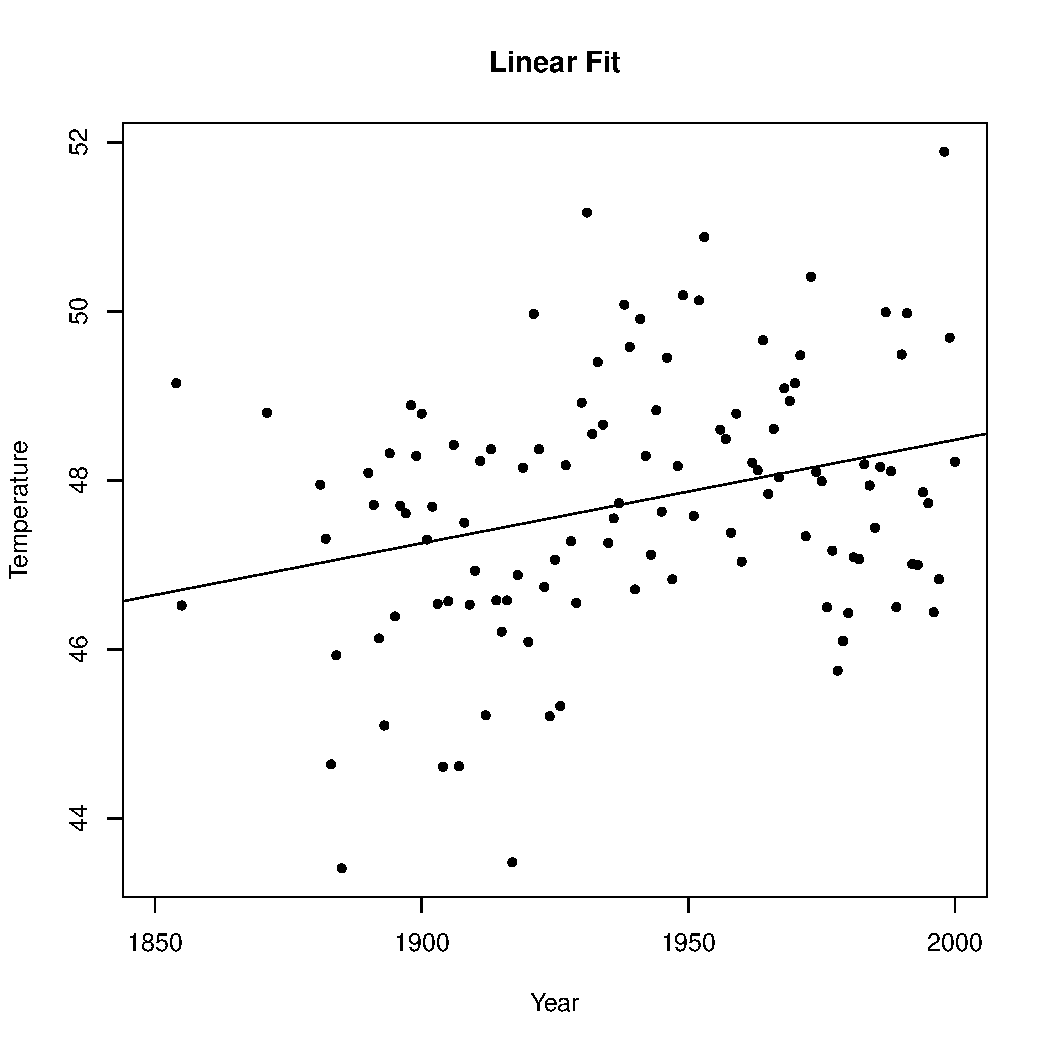
\includegraphics[width=9cm]{hw7/hw7_1_a} 
                \end{center}
            \item[b)]
                When we run a linear model that includes an AR(1) term, we find a statistically significant autoregressive term, with an estimate autocorrelation of $.208$. However, even with this, the estimates for the normal coefficients are pretty much the same as with the simple linear regression, with the coefficient on year still at $.012$ and only a small change in the intercept. The plot also shows how the plot barely changed. So, the autocorrelation  doesn't change my opinion about the trend. 
                \smallskip
                The estimate of autocorrelation:
                \FloatBarrier
                % latex table generated in R 3.1.1 by xtable 1.7-4 package
% Tue Nov 25 19:32:37 2014
\begin{table}[ht]
\centering
\begin{tabular}{rrrr}
  \hline
 & lower & est. & upper \\ 
  \hline
Phi1 & 0.012 & 0.208 & 0.389 \\ 
   \hline
\end{tabular}
\end{table}
 
                \FloatBarrier
                The estimate of coefficients:
                \FloatBarrier
                % latex table generated in R 3.1.1 by xtable 1.7-4 package
% Tue Nov 25 19:32:37 2014
\begin{table}[ht]
\centering
\begin{tabular}{rrrrr}
  \hline
 & Value & Std.Error & t-value & p-value \\ 
  \hline
(Intercept) & 25.049 & 8.759 & 2.860 & 0.005 \\ 
  year & 0.012 & 0.005 & 2.592 & 0.011 \\ 
   \hline
\end{tabular}
\end{table}
 
                \FloatBarrier
                \begin{center}
                    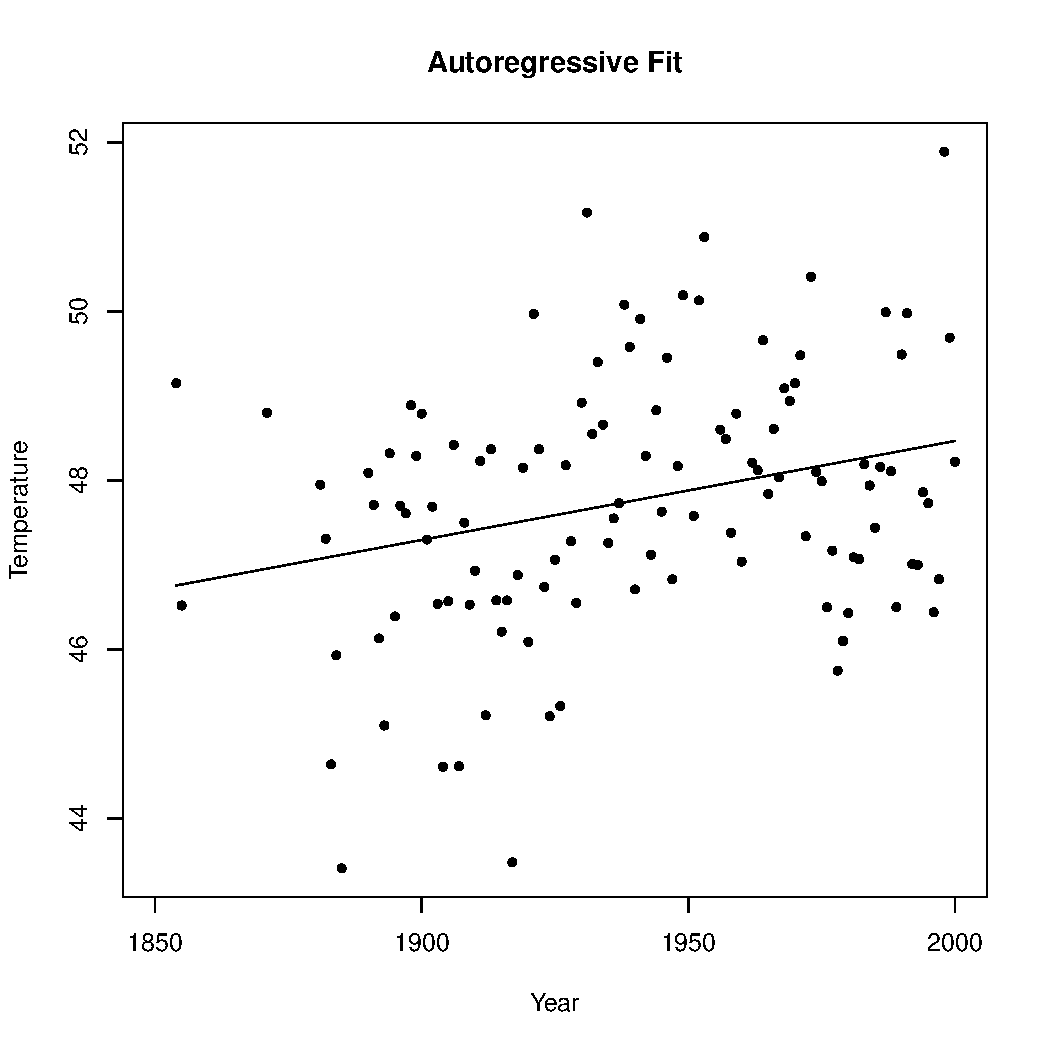
\includegraphics[width=9cm]{hw7/hw7_1_b} 
                \end{center}

            \item[c)]
                Starting with orthogonal polynomials of degree one through ten and backwards eliminating them with a critical value of $.2$, I we end up left with polynomials of degree one through five. The coefficients and plot are below. Looking at the plot, the model seems to fit quite well within the range of the data, but when we predict out to $2020$, we get a prediction of $60.078$, which is way outside of the range seen historically and thus not believable. This reflects the issues with polynomials only being a good representation of arbitrary functions where there is data to fit them.

                \smallskip
                Predicted value and range:
                \FloatBarrier
                % latex table generated in R 3.1.1 by xtable 1.7-4 package
% Tue Nov 25 19:32:37 2014
\begin{table}[ht]
\centering
\begin{tabular}{rrrr}
  \hline
 & fit & lwr & upr \\ 
  \hline
1 & 60.078 & 49.841 & 70.315 \\ 
   \hline
\end{tabular}
\end{table}
 
                \FloatBarrier               

                Estimated coefficients:
                \FloatBarrier
                % latex table generated in R 3.1.1 by xtable 1.7-4 package
% Tue Nov 25 19:32:37 2014
\begin{table}[ht]
\centering
\begin{tabular}{rrrrr}
  \hline
 & Estimate & Std. Error & t value & Pr($>$$|$t$|$) \\ 
  \hline
(Intercept) & 47.743 & 0.131 & 365.604 & 0.000 \\ 
  temp.poly.1 & 4.762 & 1.400 & 3.400 & 0.001 \\ 
  temp.poly.2 & -0.907 & 1.400 & -0.648 & 0.519 \\ 
  temp.poly.3 & -3.313 & 1.400 & -2.366 & 0.020 \\ 
  temp.poly.4 & 2.438 & 1.400 & 1.741 & 0.084 \\ 
  temp.poly.5 & 3.382 & 1.400 & 2.415 & 0.017 \\ 
   \hline
\end{tabular}
\end{table}
 
                \FloatBarrier
                \begin{center}
                    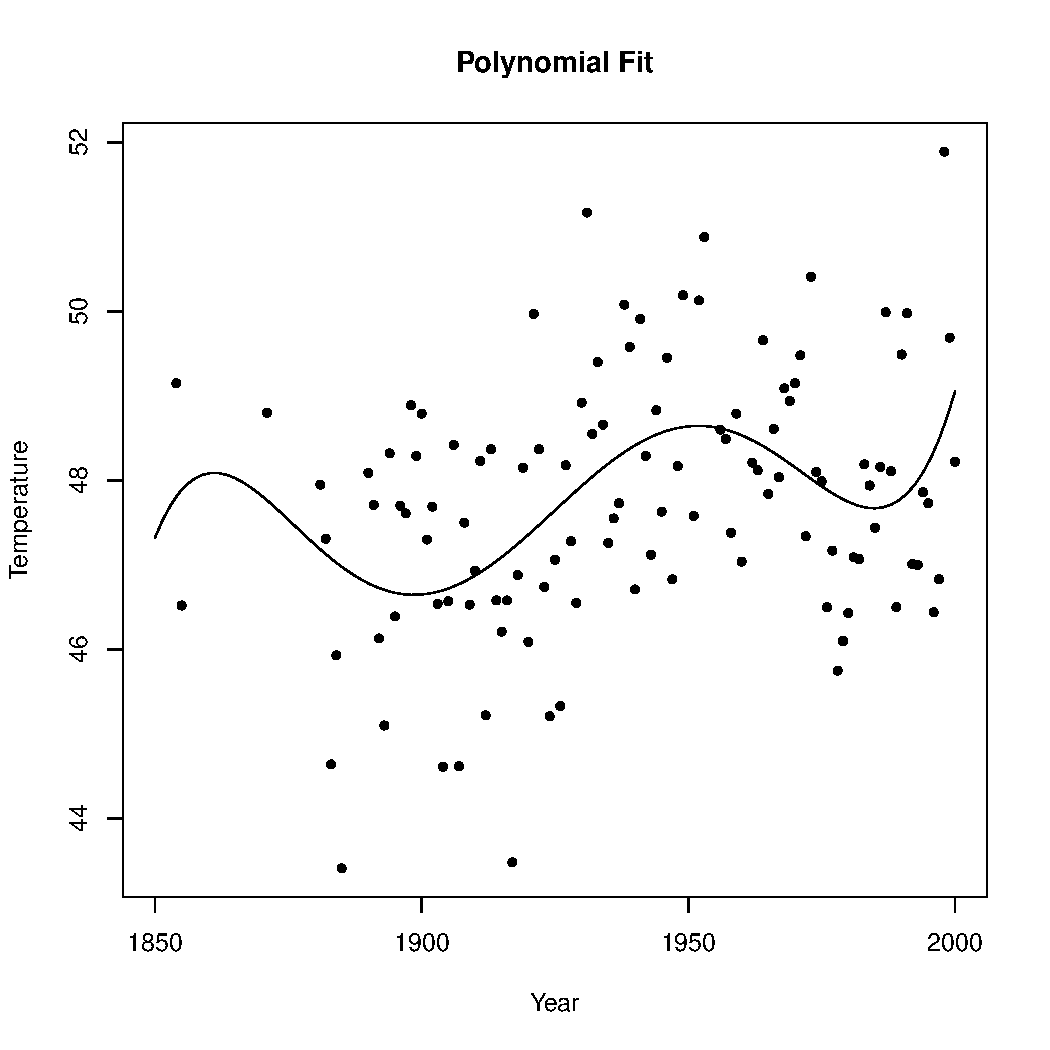
\includegraphics[width=9cm]{hw7/hw7_1_c} 
                \end{center}

            \item[d)]
                To test this trend, we fit a simple linear spline on the data, with an intercept and a continuous term for year which is $0$ before 1930. Looking at the results, we get a statistically significant coefficient on year after 1930. However, this coefficient is pretty close to the coefficient on year we had in the simple linear model, and the fit, when plotted, looks like a less convincing fit than the original simple linear model, with the actual values not symmetrically distributed around the prediction in the flat section. We don't have a formal statistical test to reject this model, but it certainly doesn't seem like an improvement over the simple linear model.

                \smallskip
                Estimated coefficients:
                \FloatBarrier
                % latex table generated in R 3.1.1 by xtable 1.7-4 package
% Tue Nov 25 19:32:37 2014
\begin{table}[ht]
\centering
\begin{tabular}{rrrrr}
  \hline
 & Estimate & Std. Error & t value & Pr($>$$|$t$|$) \\ 
  \hline
(Intercept) & 47.432 & 0.185 & 256.939 & 0.000 \\ 
  ifelse(year $<$ 1930, 0, year - 1930) & 0.015 & 0.006 & 2.556 & 0.012 \\ 
   \hline
\end{tabular}
\end{table}
 
                \FloatBarrier
                \begin{center}
                    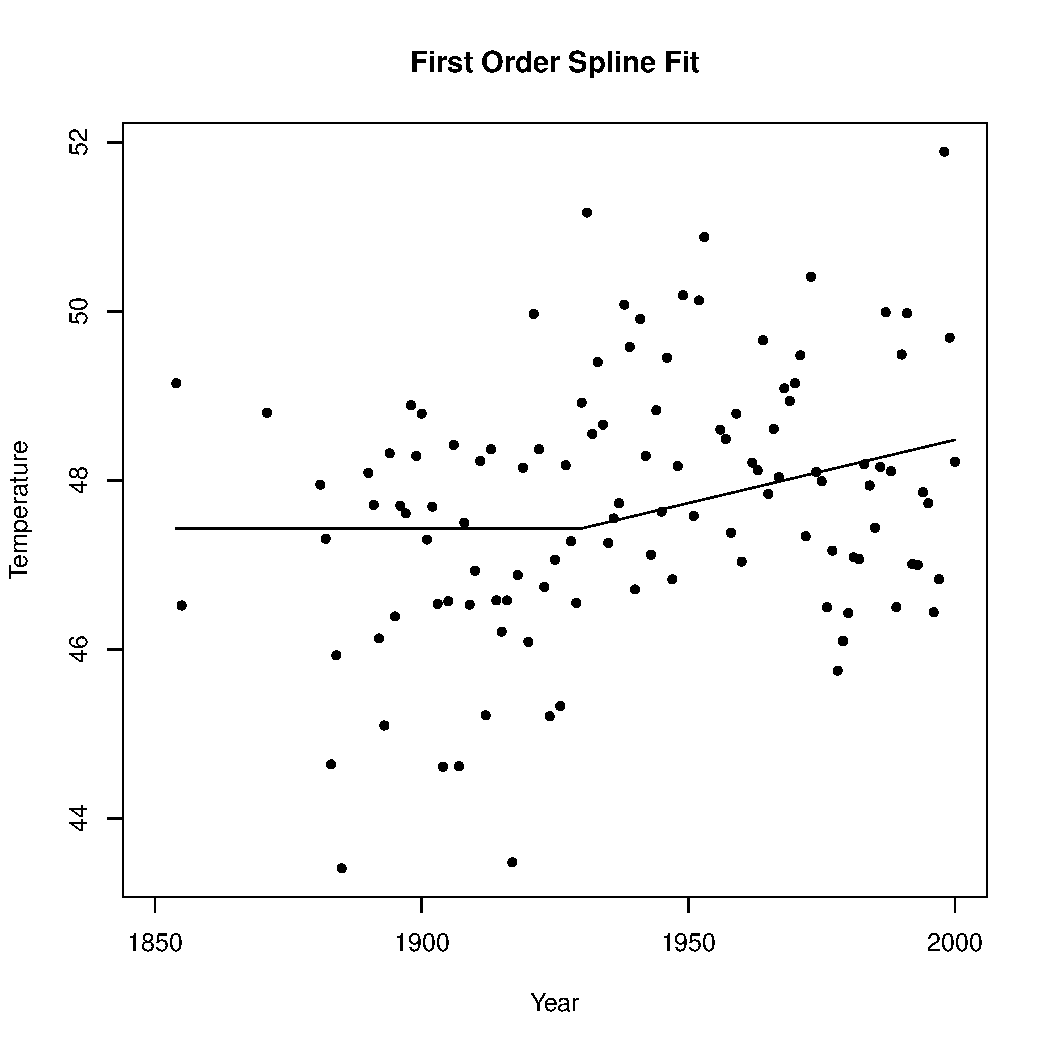
\includegraphics[width=9cm]{hw7/hw7_1_d} 
                \end{center}

            \item[e)]
                Fitting a cubic spline model, we certainly seem to see an improvement over the simple linear model. It picks up the apparent concavity over most of the 20th century, and also seems to capture the behavior towards the boundary reasonably, besides possibly turning up too sharply at the high end of the domain. Its fit is fairly similar to the polynomial fit though, with the exception of not having an inflection point on the lower end of the domain. There isn't much data in that section though, so it looks more like the polynomial is over fitting than the cubic splines.

                \smallskip
                Estimated coefficients:
                \FloatBarrier
                % latex table generated in R 3.1.1 by xtable 1.7-4 package
% Tue Nov 25 19:32:37 2014
\begin{table}[ht]
\centering
\begin{tabular}{rrrrr}
  \hline
 & Estimate & Std. Error & t value & Pr($>$$|$t$|$) \\ 
  \hline
(Intercept) & 49.275 & 0.704 & 69.954 & 0.000 \\ 
  spl1 & -1.224 & 1.246 & -0.982 & 0.328 \\ 
  spl2 & -2.151 & 1.893 & -1.136 & 0.259 \\ 
  spl3 & -2.713 & 1.130 & -2.402 & 0.018 \\ 
  spl4 & -2.081 & 1.114 & -1.868 & 0.064 \\ 
  spl5 & 0.910 & 0.907 & 1.003 & 0.318 \\ 
  spl6 & -3.228 & 1.342 & -2.405 & 0.018 \\ 
   \hline
\end{tabular}
\end{table}
 
                \FloatBarrier
                \begin{center}
                    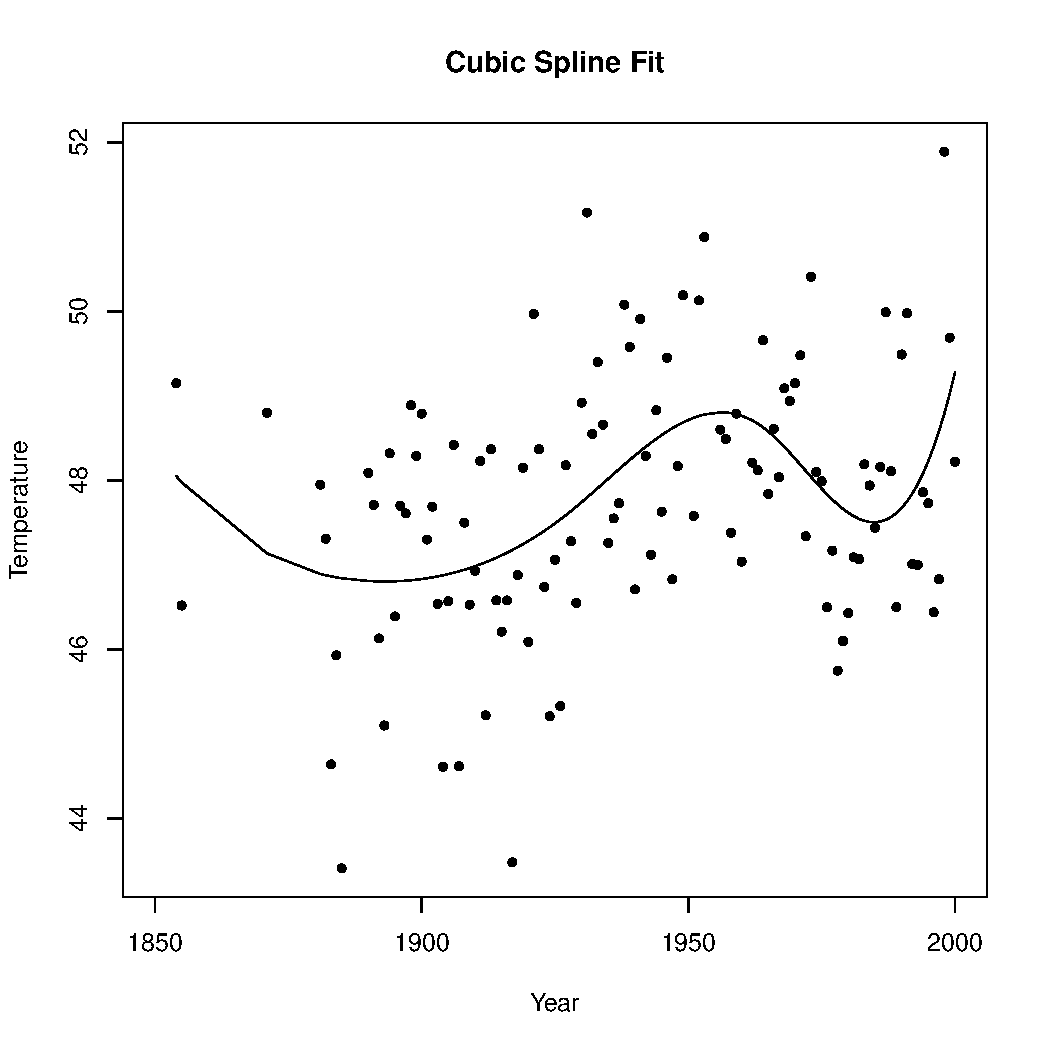
\includegraphics[width=9cm]{hw7/hw7_1_e} 
                \end{center}
        \end{itemize}
    \item[2.]
        \begin{itemize}
            \item[a)]
                After running the model on the untransformed data, we seem to see a substantial improvement from transformation. The log-likelihood for box-cox is maximized right around $\lambda=.25$, with a confidence interval that excluded $1$, so I transformed the data using $.25$. The end result is an improvement in $R^2$ from $.681$ to $.713$.
                \smallskip
                The untransformed linear model:
                \FloatBarrier
                % latex table generated in R 3.1.1 by xtable 1.7-4 package
% Tue Nov 25 19:32:37 2014
\begin{table}[ht]
\centering
\begin{tabular}{rrrrr}
  \hline
 & Estimate & Std. Error & t value & Pr($>$$|$t$|$) \\ 
  \hline
(Intercept) & -10.494 & 1.616 & -6.492 & 0.000 \\ 
  temp & 0.330 & 0.021 & 15.626 & 0.000 \\ 
  humidity & 0.077 & 0.013 & 5.777 & 0.000 \\ 
  ibh & -0.001 & 0.000 & -6.130 & 0.000 \\ 
   \hline
\end{tabular}
\end{table}

                \FloatBarrier                
                \begin{center}
                    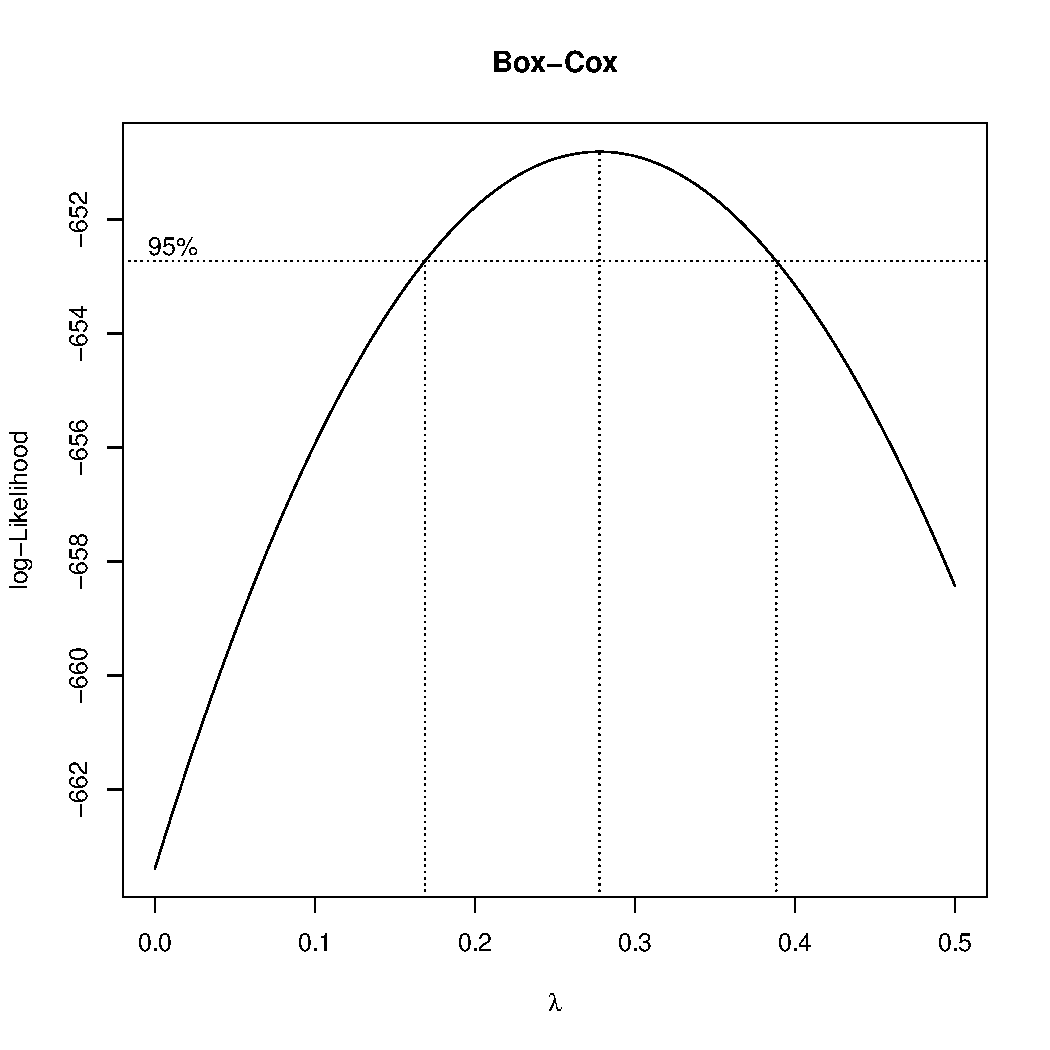
\includegraphics[width=9cm]{hw7/hw7_2_a} 
                \end{center}
                The transformed linear model:
                \FloatBarrier
                % latex table generated in R 3.1.1 by xtable 1.7-4 package
% Tue Nov 25 19:32:37 2014
\begin{table}[ht]
\centering
\begin{tabular}{rrrrr}
  \hline
 & Estimate & Std. Error & t value & Pr($>$$|$t$|$) \\ 
  \hline
(Intercept) & 0.914 & 0.062 & 14.774 & 0.000 \\ 
  temp & 0.013 & 0.001 & 16.192 & 0.000 \\ 
  humidity & 0.003 & 0.001 & 5.810 & 0.000 \\ 
  ibh & -0.000 & 0.000 & -7.734 & 0.000 \\ 
   \hline
\end{tabular}
\end{table}

                \FloatBarrier                
            \item[b)]
                Comparing the linear fit to the regression tree and the random forest, it appears that the latter two fit slightly better than the former. As we look at the residuals, both the regression tree and the random forest are nearly perfectly distributed around 0 through out the predicted range (for the random tree this is of course by construction), while the residuals for the linear model do not quite seem to be at the lower end of the predicted range. As well, while the linear model residuals deviate from a normal distribution towards the upper end of their range, the regression tree and random forest have residuals that are normally distributed pretty well throughout. \\
                \smallskip
                This is the regression tree I fit:
                \begin{center}
                    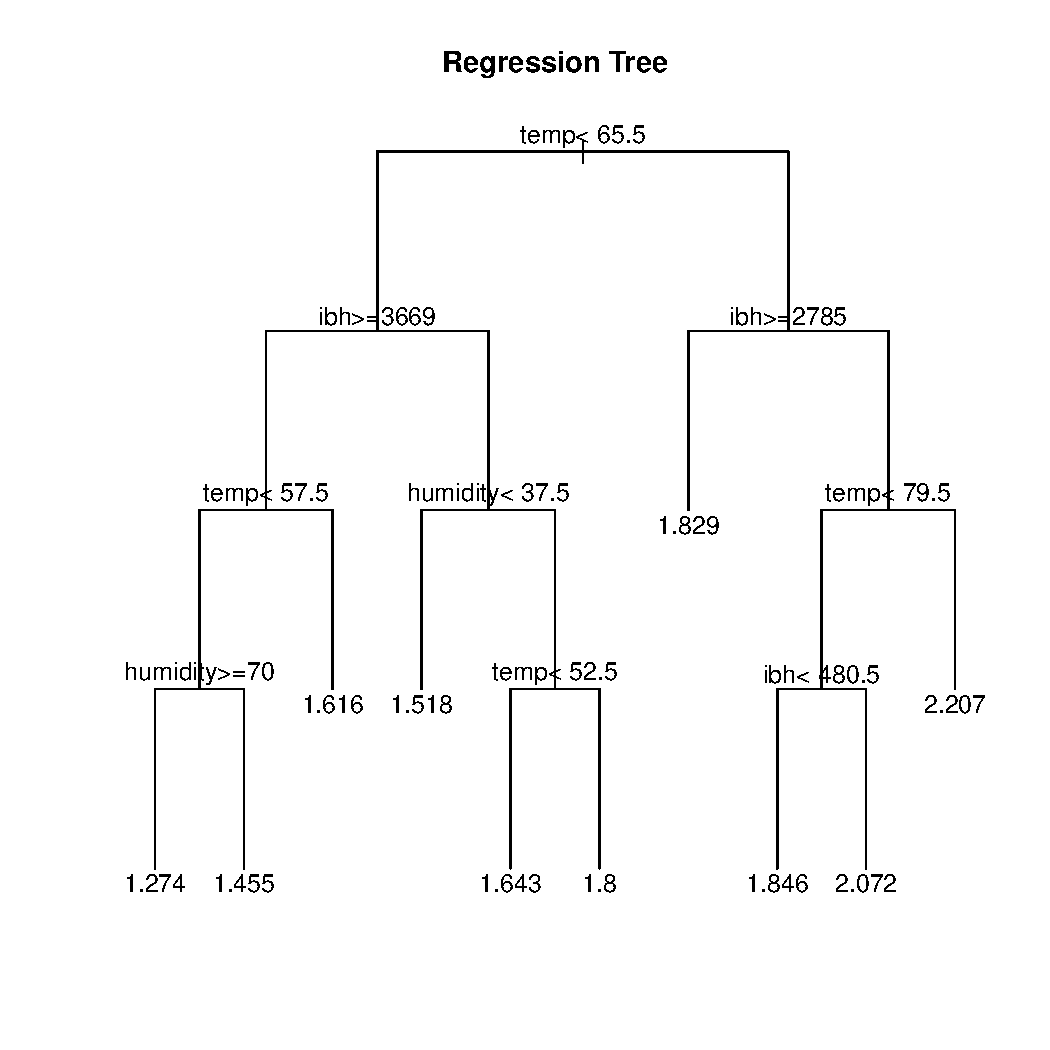
\includegraphics[width=9cm]{hw7/hw7_2_b_tree} 
                \end{center}
                The transformed linear regression: \\
                    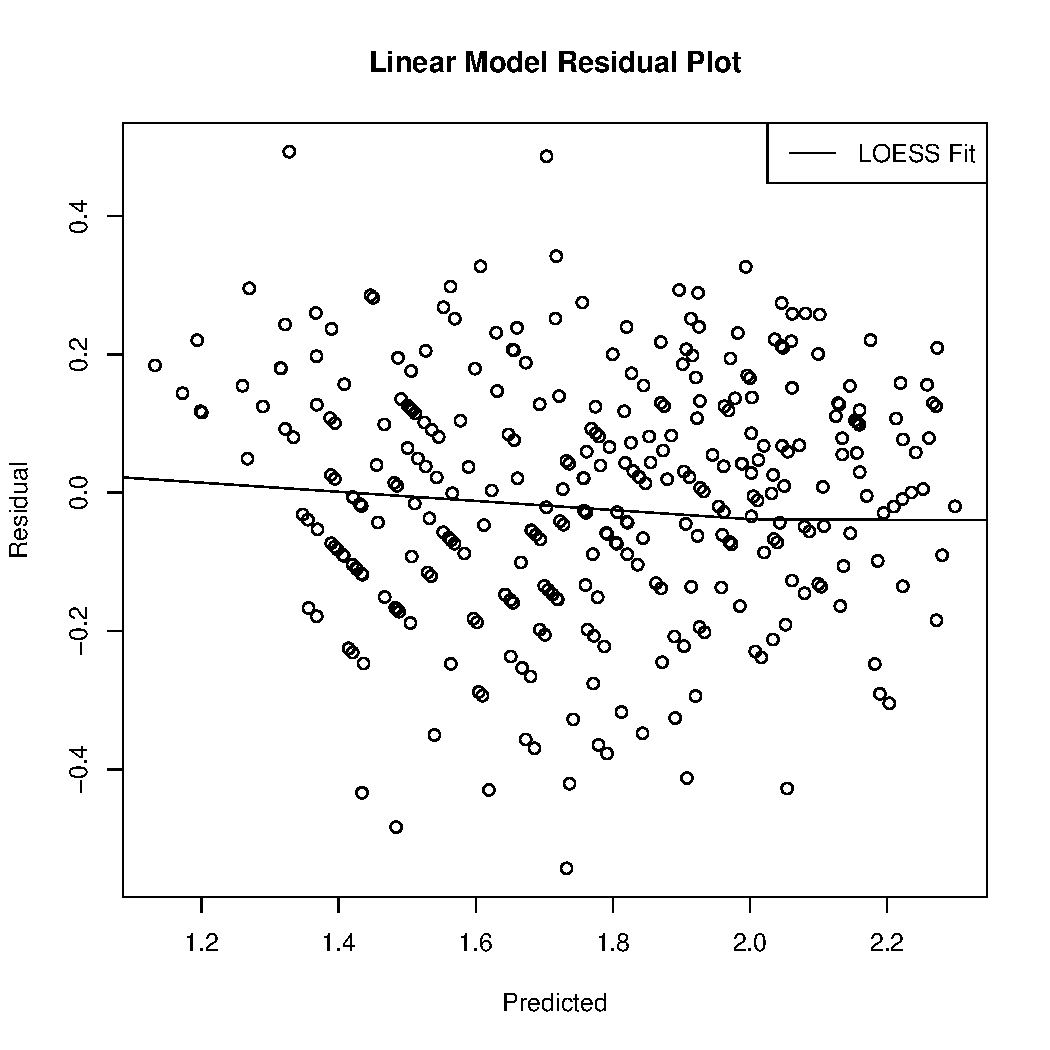
\includegraphics[width=9cm]{hw7/hw7_2_b_lm_res} 
                    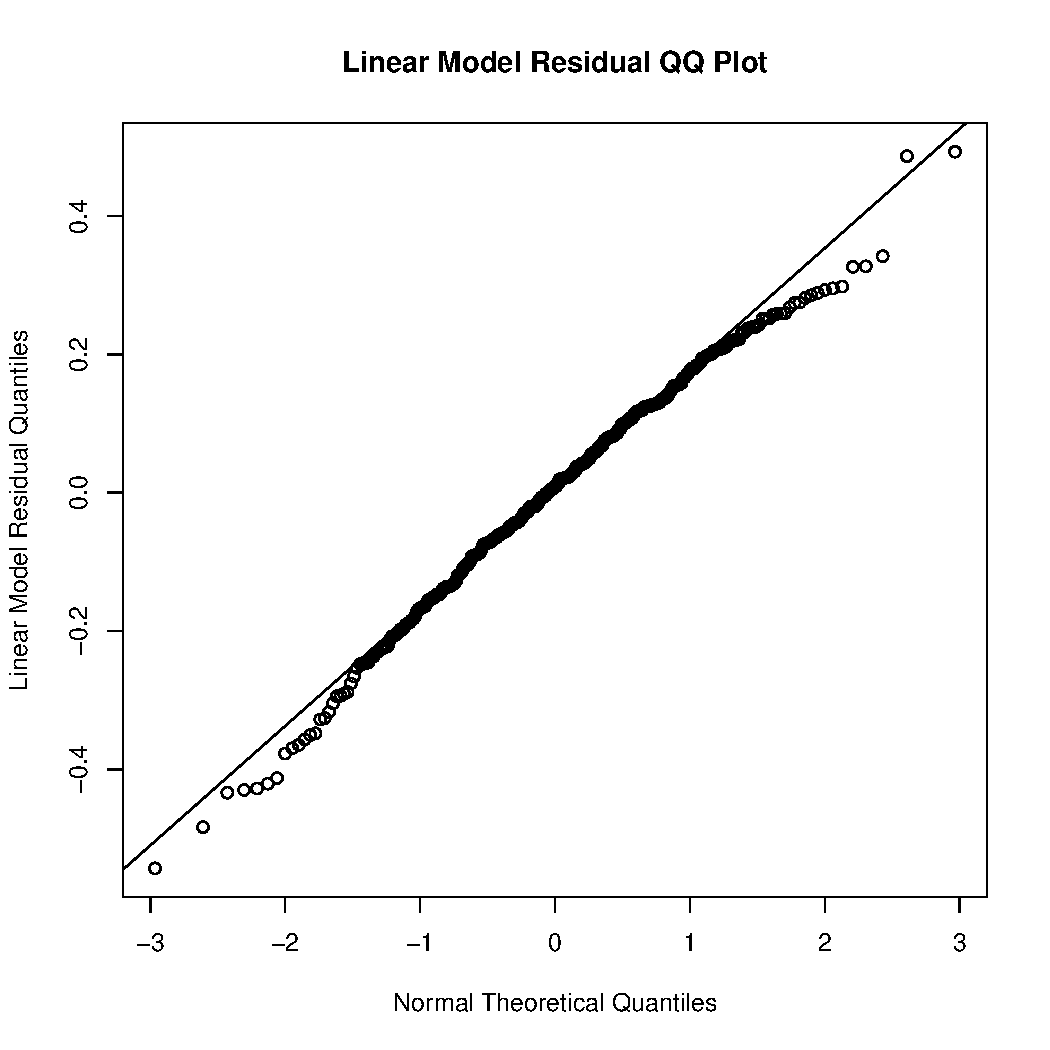
\includegraphics[width=9cm]{hw7/hw7_2_b_lm_qq} \\ 
                The regression tree: \\
                    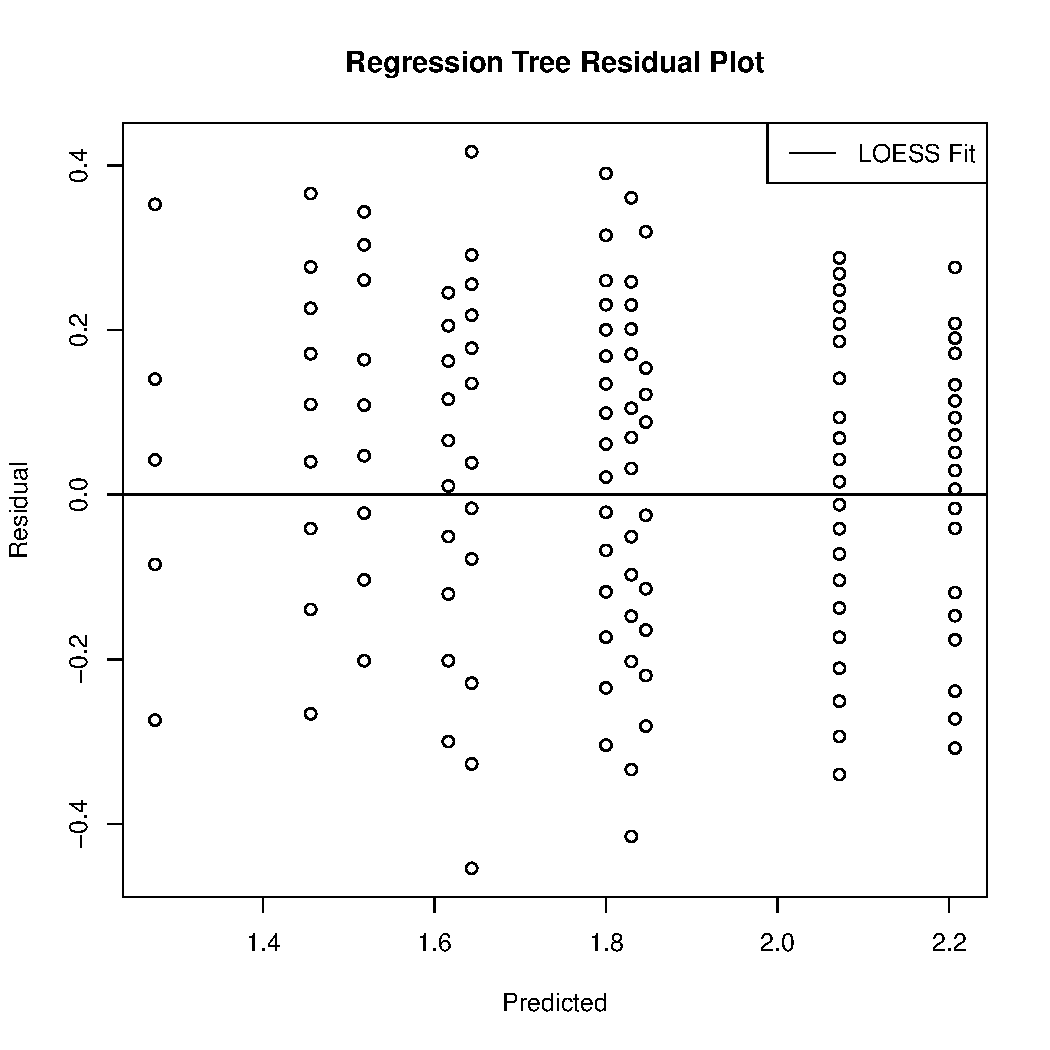
\includegraphics[width=9cm]{hw7/hw7_2_b_rt_res} 
                    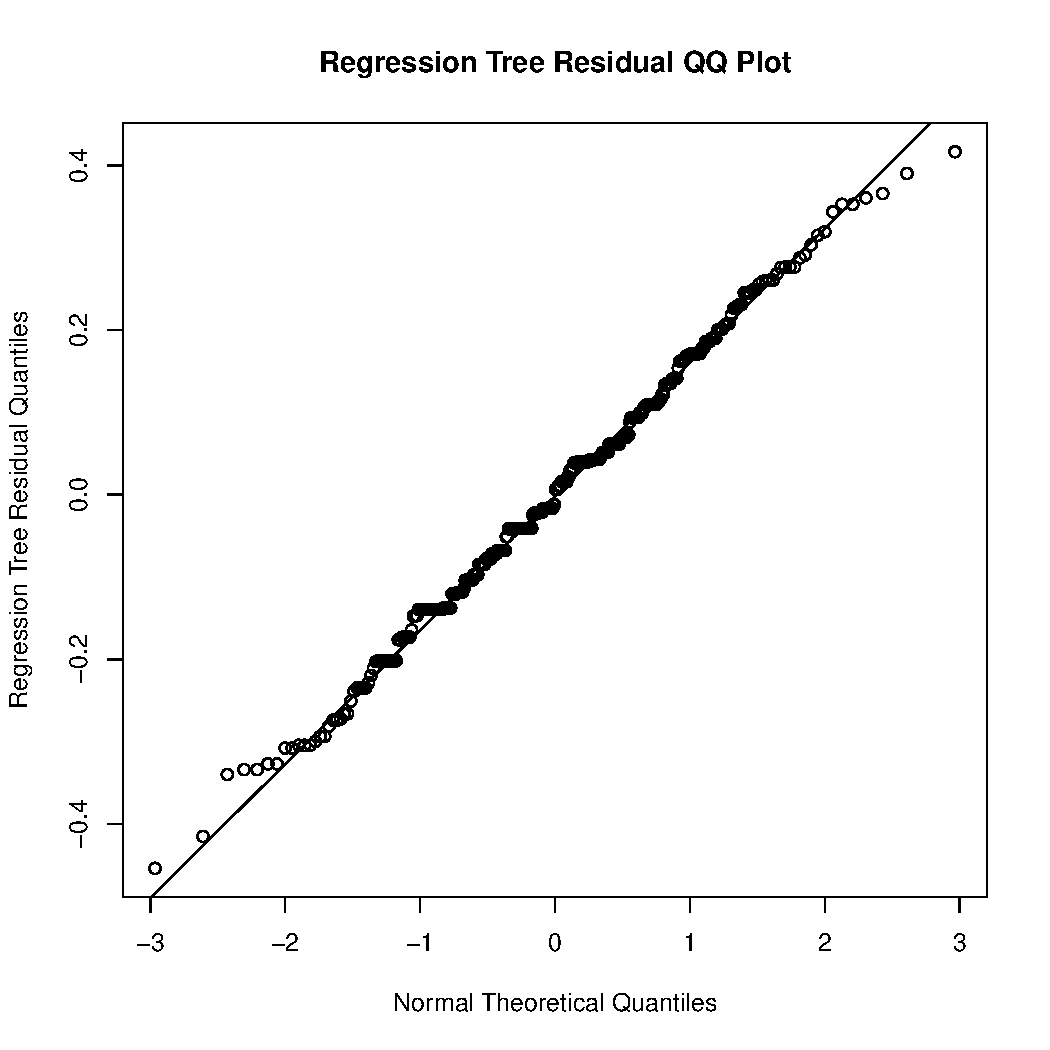
\includegraphics[width=9cm]{hw7/hw7_2_b_rt_qq} \\ 
                The random forest: \\
                    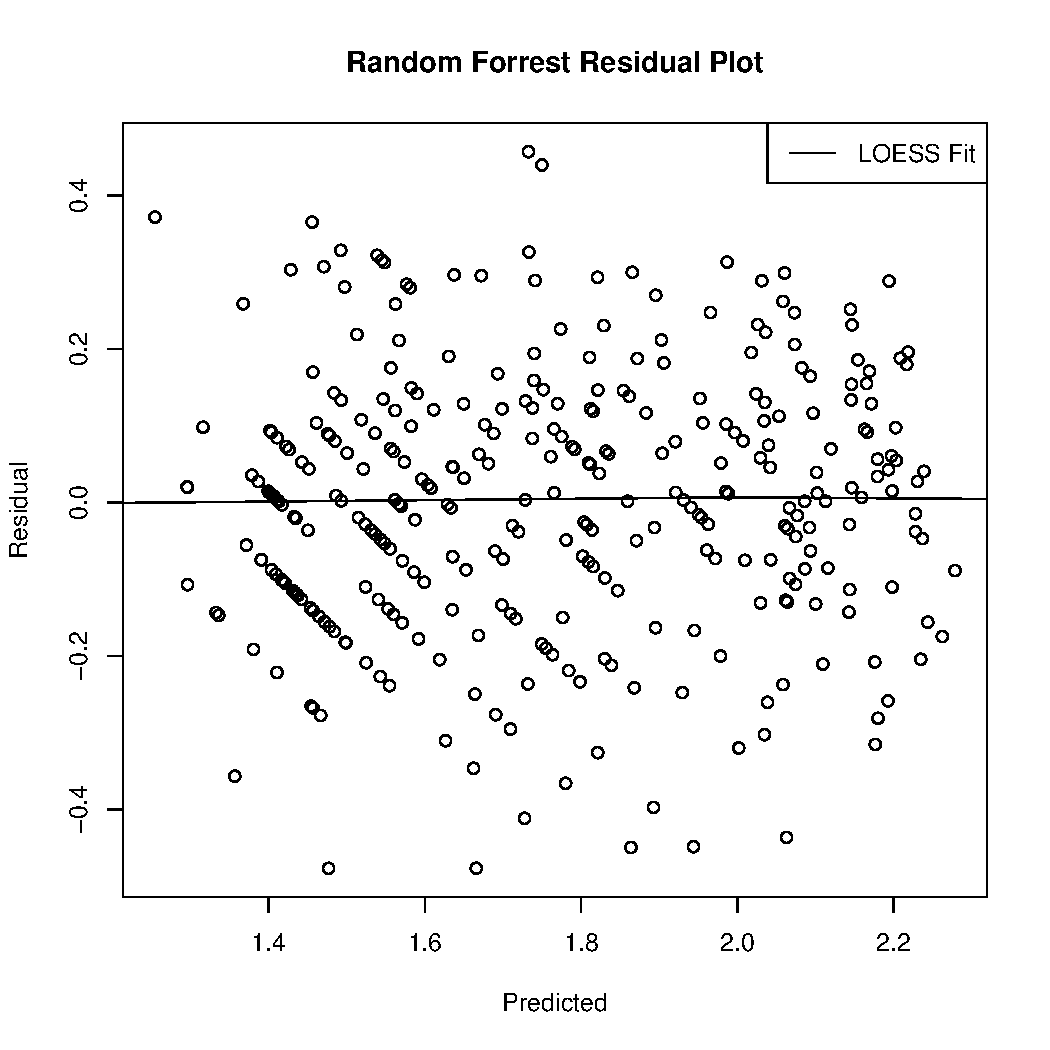
\includegraphics[width=9cm]{hw7/hw7_2_b_rf_res} 
                    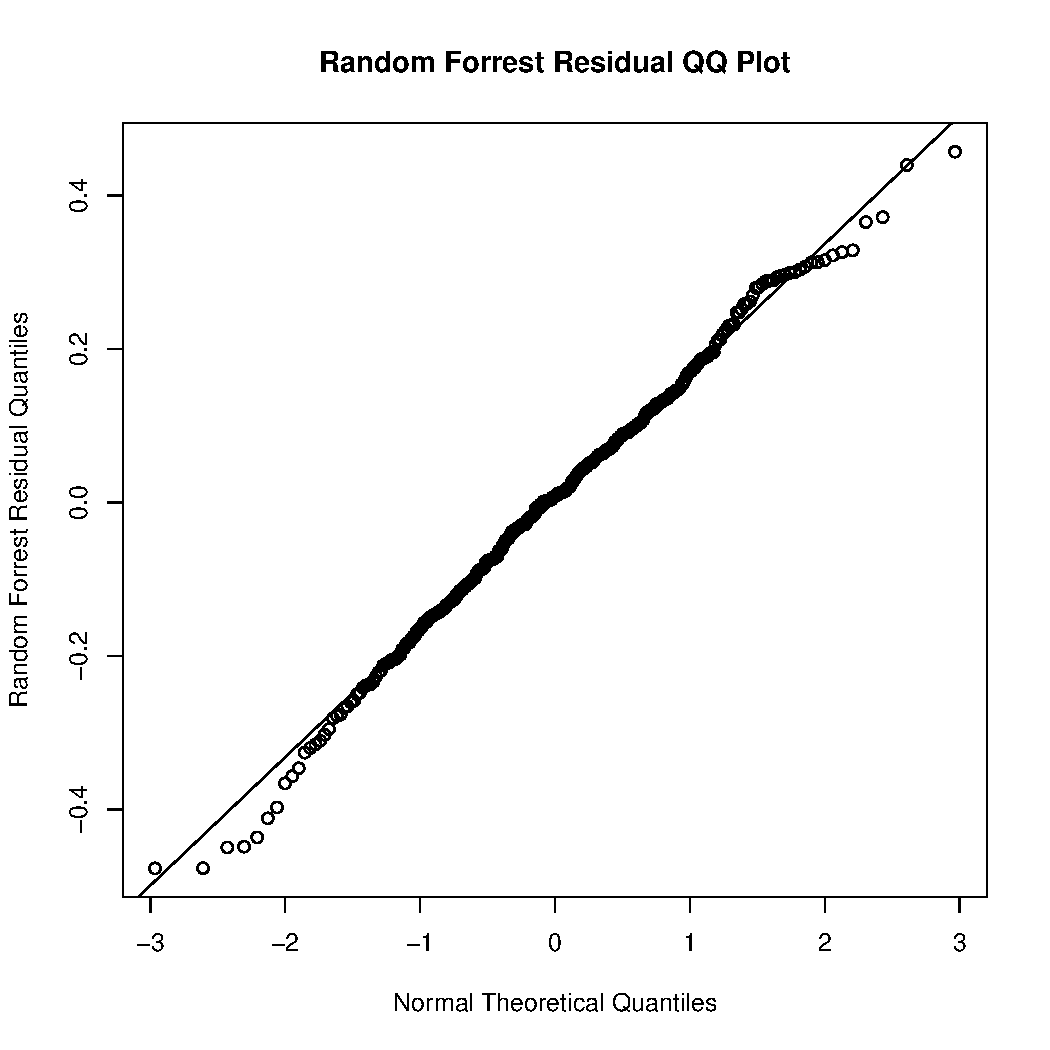
\includegraphics[width=9cm]{hw7/hw7_2_b_rf_qq} \\ 

        \end{itemize}
    \item[3.]
        \item[a)]
            I applied backwards elimination, working with a critical value of $.2$. Doing this, I eliminated three variables and kept the rest.
            \smallskip
            This was the order I eliminated variables in, and their p-value when I eliminated them:\\
            \FloatBarrier
            % latex table generated in R 3.1.1 by xtable 1.7-4 package
% Tue Nov 25 19:32:38 2014
\begin{table}[ht]
\centering
\begin{tabular}{rrr}
  \hline
 & Order & p-value \\ 
  \hline
gleason & 1.000 & 0.775 \\ 
  lcp & 2.000 & 0.251 \\ 
  pgg45 & 3.000 & 0.253 \\ 
   \hline
\end{tabular}
\end{table}

            \FloatBarrier                
            The end result was this regression: \\
            \FloatBarrier
            % latex table generated in R 3.1.1 by xtable 1.7-4 package
% Tue Nov 25 19:32:38 2014
\begin{table}[ht]
\centering
\begin{tabular}{rrrrr}
  \hline
 & Estimate & Std. Error & t value & Pr($>$$|$t$|$) \\ 
  \hline
(Intercept) & 0.951 & 0.832 & 1.143 & 0.256 \\ 
  lcavol & 0.566 & 0.075 & 7.583 & 0.000 \\ 
  lweight & 0.424 & 0.167 & 2.539 & 0.013 \\ 
  age & -0.015 & 0.011 & -1.385 & 0.170 \\ 
  lbph & 0.112 & 0.058 & 1.927 & 0.057 \\ 
  svi & 0.721 & 0.209 & 3.449 & 0.001 \\ 
   \hline
\end{tabular}
\end{table}

            \FloatBarrier                
        \item[b)]
            Going by forward selection, again with a critical value of $.2$, I ended up with the same model gotten previously by backwards selection. 
            \smallskip
            This was the order I included variables in, and their p-value when I included them:\\
            \FloatBarrier
            % latex table generated in R 3.1.1 by xtable 1.7-4 package
% Tue Nov 25 19:32:38 2014
\begin{table}[ht]
\centering
\begin{tabular}{rrr}
  \hline
 & Order & p-value \\ 
  \hline
lcavol & 1.000 & 0.000 \\ 
  lweight & 2.000 & 0.002 \\ 
  svi & 3.000 & 0.002 \\ 
  lbph & 4.000 & 0.112 \\ 
  age & 5.000 & 0.170 \\ 
   \hline
\end{tabular}
\end{table}

            \FloatBarrier                
            The end result was this regression: \\
            \FloatBarrier
            % latex table generated in R 3.1.1 by xtable 1.7-4 package
% Tue Nov 25 19:32:38 2014
\begin{table}[ht]
\centering
\begin{tabular}{rrrrr}
  \hline
 & Estimate & Std. Error & t value & Pr($>$$|$t$|$) \\ 
  \hline
(Intercept) & 0.951 & 0.832 & 1.143 & 0.256 \\ 
  lcavol & 0.566 & 0.075 & 7.583 & 0.000 \\ 
  lweight & 0.424 & 0.167 & 2.539 & 0.013 \\ 
  svi & 0.721 & 0.209 & 3.449 & 0.001 \\ 
  lbph & 0.112 & 0.058 & 1.927 & 0.057 \\ 
  age & -0.015 & 0.011 & -1.385 & 0.170 \\ 
   \hline
\end{tabular}
\end{table}

            \FloatBarrier                

    \item[4.]
        As I think we had to show on the midterm,
        \begin{align*}
            H&= X(X^TX)^{-1}X^T \\
            H&= QR(R^TQ^TQR)^{-1}R^TQ^T \\
            H&= QR(R^TR)^{-1}R^TQ^T \\
            H&= QRR^{-1}(R^T)^{-1}R^TQ^T \\
            H&= QQ^T
        \end{align*}
        As was discussed with added variable plots, for an additional variable $X_i$ added to a regression, if $\hat e_{(-i)}$ are the residuals from the regression excluding $X_i$, $\hat e$ are the residuals from the regression including it, and $\beta_i$ is what the coefficient would be on $X_i$ if it was included in the regression, then
        \begin{align*}
            \hat e_{(-i)} &= \hat\beta_i (I-H) X_i + \hat e \\ 
            \hat e_{(-i)} &= \hat\beta_i (I-QQ^T) X_i + \hat e \\ 
        \end{align*}
        From simple linear regression, since \(\hat e_{(-i)}\) has mean $0$, it must be the case that \(\hat\beta_i=\frac{\cov((I-QQ^T) X_i,\hat e_{(-i)})}{\var((I-QQ^T) X_i)}\). Plugging this in, we get
        \begin{align*}
            \hat e_{(-i)} &= \frac{\cov((I-QQ^T) X_i,e_{(-i)})}{\var((I-QQ^T) X_i)} (I-QQ^T) X_i + \hat e \\ 
            \hat e &= \hat e_{(-i)} - \frac{\cov\left((I-QQ^T) X_i,\hat e_{(-i)}\right)}{\var\left((I-QQ^T) X_i\right)} (I-QQ^T) X_i \\ 
            \|\hat e\|^2 &= \left\|\hat e_{(-i)} - \frac{\cov\left((I-QQ^T) X_i,\hat e_{(-i)}\right)}{\var\left((I-QQ^T) X_i\right)} (I-QQ^T) X_i \right \|^2 \\
            RSS &= \left\|\hat e_{(-i)} - \frac{\cov\left((I-QQ^T) X_i,\hat e_{(-i)}\right)}{\var\left((I-QQ^T) X_i\right)} (I-QQ^T) X_i \right \|^2
        \end{align*}
        Thus, we can minimize the $RSS$ by choosing the variable $X_i$ such that the quantity on the right is minimized.
    \item[5.]
        $RSS$ will be increased the least by removing the variable which has the highest p-value. \\
        \smallskip
        {\bf Explanation:} If $RSS_{(-i)}$ is the residual sum of squares for a model excluding variable $i$, we want to pick $i$ such that $RSS_{(-i)}-RSS$ is smallest. Obviously, the same $i$ will minimize
        \[ F= \frac{\frac{RSS_{(-i)}-RSS}{p-(p-1)}}{\frac{RSS}{n-p}}\]
        This will in turn maximize the p-value for the F test comparing the model to the model excluding variable $i$. However, as we know, this p-value is equivalent to the p-value from the t test in the regression summary for variable $i$. Thus, this variable, when removed, will result in the smallest increase in $RSS$.

\end{itemize}
\end{document}
